\documentclass[11pt]{article}
\usepackage[margin=1in]{geometry}
\usepackage{graphicx,booktabs,hyperref,float,subcaption,xcolor,array,enumitem,amsmath}
\setlength{\parskip}{0.5em}\setlength{\parindent}{0pt}
\title{Parametric IFC Design Studio\\\large How requirements, zoning and BaaP rules become a viewable building}
\author{RNGD side-testing project}
\date{\today}
\begin{document}
\maketitle
\tableofcontents

\section{Summary}
This test answers one question: \emph{can we go from customer requirements, zoning rules and a catalog of standard building modules to a real
3D building file, using only free, open-source tools?} The answer is yes. A Python program reads the requirements, applies a zoning preset and the
BaaP (Building-as-a-Product) module catalog, lays out a building, and writes it as a standard \textbf{IFC4} file using \textbf{IfcOpenShell}. The file
is then re-read from disk and displayed in Chrome as an interactive 3D model, with buttons and sliders that regenerate the design instantly. Every
design is scored against ten pass/fail checks so you can see why a design works or fails.

Three important honesty notes. (1) All zoning rules and BaaP module data are \textbf{synthetic samples}; they stand in for RNGD's real data. (2) The layout is
\textbf{planning-level}: it is a rule-based massing and unit layout, not a code-approved drawing set. (3) No Revit file (\texttt{.rvt}) is produced; that
step was dropped from scope. The IFC opens in free BIM tools instead.

\section{Background: the terms used in this report}
\begin{description}[leftmargin=4.5cm,style=nextline]
\item[IFC (Industry Foundation Classes)] The open, vendor-neutral file format for building models (ISO 16739). It stores real building objects
(walls, slabs, storeys) with geometry and names, not just pictures. Most BIM software can open it.
\item[IfcOpenShell] A free Python library that creates, reads and triangulates IFC files. We use it both to write the design and to read it back.
\item[BaaP (Building-as-a-Product)] RNGD's idea of building from a fixed catalog of standard modules (unit types, cores, corridors) instead of designing each
building from scratch. Here the catalog is in \texttt{data/baap\_catalog.json}.
\item[Setback] The strip along each lot edge where building is not allowed. \textbf{Easement:} a strip reserved for utilities, also unbuildable.
\item[Buildable envelope] The rectangle left after removing setbacks and easements. Everything must fit inside it.
\item[FAR (floor area ratio)] Total building floor area divided by lot area. Limits how much building you can put on a lot.
\item[Lot coverage] Building footprint area divided by lot area, as a percent.
\item[Double-loaded corridor] A hallway with unit modules on both sides; the most efficient way to pack apartments.
\item[Core] The block with stairs, elevator and shafts that serves the corridor. \textbf{Wing:} one long bar of corridor plus units. A building may have one to three wings.
\item[Podium parking] A parking level built into the base of the building, instead of surface stalls, used when the lot is too small for surface parking.
\end{description}

\section{System overview}
The data flow is a straight line from requirements to a file you can open:
\[
\text{requirements} + \text{zoning preset} + \text{BaaP catalog}
\;\rightarrow\; \texttt{design.py}
\;\rightarrow\; \texttt{ifc\_writer.py}
\;\rightarrow\; \texttt{.ifc}
\;\rightarrow\; \texttt{viewer3d.py}
\;\rightarrow\; \text{Chrome}
\]
\begin{table}[H]\centering\small
\begin{tabular}{@{}lp{10.5cm}@{}}\toprule
File & Job \\ \midrule
\texttt{design.py} & Holds the zoning presets and parameters; computes the envelope, packs units, places driveway and parking, and runs the ten compliance checks. Pure Python, all dimensions in feet. \\
\texttt{ifc\_writer.py} & Converts a layout to an IFC4 file (metres) and also reads an IFC back into triangle meshes. \\
\texttt{viewer3d.py} & Turns the meshes into an interactive Plotly 3D figure, colored by unit type. \\
\texttt{app.py} & The Streamlit browser app: buttons, sliders, tabs, downloads. Optionally uses the existing AI intake agent to parse a pasted customer request. \\
\texttt{generate.py} & Command-line tool that writes every scenario to \texttt{out/} as \texttt{.ifc} and a standalone \texttt{.html} viewer. \\
\texttt{test\_design.py} & 12 automated tests. \texttt{build\_report.py} builds this document. \\ \bottomrule
\end{tabular}\end{table}

\section{Inputs in detail}
\subsection{Requirements (what the customer wants)}
These are fields of the \texttt{Params} object and the app's sidebar controls.
\begin{table}[H]\centering\small
\begin{tabular}{@{}llp{8cm}@{}}\toprule
Input & Default & Meaning \\ \midrule
Units & 120 & Total apartments requested (a hard requirement in the sample request). \\
Unit mix & 20/45/35\,\% & Share of studio, 1-bedroom, 2-bedroom units. \\
Residential floors & 4 & Number of floors that contain apartments. \\
Parking type & surface & \texttt{surface} stalls on the ground, or \texttt{podium} parking under the building. \\
Wings & auto & 0 lets the program try 1, 2 and 3 wings and pick the best; 1--3 forces a choice. \\
Lot & 200$\times$300\,ft & Frontage $\times$ depth; street at the top; 20\,ft utility easement on the east side. \\
Story heights & 14 / 10.5\,ft & Ground (or podium) level and typical upper level. \\ \bottomrule
\end{tabular}\end{table}
In the app, a free-text request can be pasted and the AI intake agent (Groq) extracts units, floors and mix into these controls automatically.

\subsection{Zoning presets (the rules)}
Three synthetic presets are included so you can see how the same building behaves under different rules. Setbacks are front/side/rear in feet.
\begin{table}[H]\centering\small
\begin{tabular}{lllllll}\toprule
Preset & Setbacks & FAR & Cov.\,\% & Height & Stories & Parking/unit \\ \midrule
Rivermont R-4 (sample) & 15/10/20 & 2.5 & 60 & 65 & 5 & 1.25 \\
Dense urban R-6 (sample) & 10/5/15 & 3.5 & 75 & 85 & 7 & 0.75 \\
Suburban R-2 (sample) & 25/10/25 & 1.0 & 40 & 35 & 3 & 2.0 \\
\bottomrule\end{tabular}\end{table}

\subsection{BaaP catalog (the building blocks)}
Unit modules are fixed products; the design problem is choosing how many of each and where they go.
\begin{table}[H]\centering\small
\begin{tabular}{lllll}\toprule
Module & Type & Width $\times$ depth (ft) & GSF & Notes \\ \midrule
STUDIO\_A & Studio & 26 $\times$ 32 & 550 & \\
ONEBR\_A & 1-bedroom & 30 $\times$ 34 & 725 & \\
TWOBR\_A & 2-bedroom & 34 $\times$ 36 & 1020 & \\
ACCESSIBLE\_1BR & 1-bedroom (ADA) & 32 $\times$ 34 & 760 & counted for the 2\% rule \\
CORE\_STD & Stairs + elevator core & 24 along corridor $\times$ 34 across & -- & one per wing per floor \\
Amenities & Lobby, fitness, loading & 1200 / 900 / 600 GSF & -- & ground floor only \\ \bottomrule
\end{tabular}\end{table}

\section{How the layout is generated}
This is the heart of the program. Each step is deterministic: the same inputs always give the same building.

\subsection{Step 1: buildable envelope}
With side setback $s$, front $f$, rear $r$, easement $e$ on the east, and lot $W\times D$:
\[
x_0 = s,\quad x_1 = W - \max(s, e),\quad y_0 = f,\quad y_1 = D - r .
\]
The easement replaces the side setback on that side because it is wider. For the baseline: $x_0=10$, $x_1=200-20=180$, $y_0=15$, $y_1=300-20=280$, so the envelope is
\textbf{170\,ft $\times$ 265\,ft = 45,050\,sf}.

\subsection{Step 2: how many of each unit}
Studios and one-bedrooms are $\text{round}(N\times\text{share})$; two-bedrooms get the remainder so the total is exactly $N$. For 120 units this gives
24 studios, 54 one-bedrooms and 42 two-bedrooms.

\subsection{Step 3: spreading the unit types evenly}
A proportional interleave decides the order of units along a corridor so studios, one- and two-bedrooms are mixed evenly rather than grouped. For step $i$ of $N$, it
picks the type with the largest gap between its target count $c_k\cdot i/N$ and the number already used. This is the same idea as largest-remainder apportionment.

\subsection{Step 4: the shape of one wing}
The bar's width is two rows of the deepest unit plus a corridor: $2\times 36 + 6 = 78$\,ft. A core (24\,ft along the corridor, 34\,ft across) sits at the
start of each wing. Wings run along the \emph{longer} side of the envelope (here the 265\,ft depth). Several wings sit side by side with a 10\,ft gap. A 24\,ft driveway
is placed on the west side if the wings plus 24\,ft still fit across the envelope; otherwise the program tries a lane across the far end of the wings.

\subsection{Step 5: storeys and heights}
With surface parking, level 1 is 14\,ft and upper levels 10.5\,ft. With podium parking an extra 14\,ft parking level sits below level 1, and residential levels are 10.5\,ft.
The building height is the sum of storey heights; the roof is a zero-height marker storey at the top.

\subsection{Step 6: packing units floor by floor}
Each wing has two rows (one each side of the corridor). Floor by floor, the program places units greedily:
\begin{enumerate}[nosep]
\item Compute how many units this floor should take: $\lceil \text{units remaining} / \text{floors remaining}\rceil$, so units spread evenly.
\item On level 1, the lobby, fitness room and loading area (width $=$ GSF$/24$\,ft) take space at the start of the first row of wing 1, so fewer units fit on the ground floor.
\item For each next unit in the interleaved order, choose the row with the shortest used length (so rows balance), and place the unit if it fits.
\item Units are aligned to the corridor edge, so different depths line up along the hallway.
\end{enumerate}
A wing's final length is the longest row length reached on any floor, so the wing is only as long as it needs to be. If units do not fit within the envelope length, the leftover
units are reported as \emph{not placed}.

\subsection{Step 7: accessible units}
The rule needs $\max(1,\lceil 0.02\,N\rceil)$ accessible units. The first that many one-bedroom units are converted to ACCESSIBLE\_1BR (3 units for 120, 2 for 60).

\subsection{Step 8: parking}
\emph{Required stalls} $=\lceil \text{ratio}\times N\rceil$ (150 for 120 units at 1.25). For \textbf{surface} parking the program scans rows of $9\times18$\,ft stalls, 42\,ft apart (18\,ft stall
plus 24\,ft aisle), inside the envelope, skipping any stall that touches a wing or the driveway, until the requirement is met or space runs out. For \textbf{podium} parking the capacity is estimated as
$0.85\times\text{footprint}/330$\,sf per stall (85\,\% usable, 330\,sf per stall including aisles), and surface stalls only cover what podium cannot.

\subsection{Step 9: choosing the number of wings}
When wings is set to auto, the program builds designs with 1, 2 and 3 wings and keeps the best by a ranked score: (1) all units placed, (2) building inside the envelope, (3) a fire lane exists, (4) fewer wings.

\section{The ten compliance checks}
Each check gives PASS or FAIL so the reason for a failure is visible.
\begin{table}[H]\centering\small
\begin{tabular}{@{}lp{9cm}@{}}\toprule
Check & Rule used \\ \midrule
Units placed & Placed units $\ge$ requested units. \\
Stories & Storeys (including a podium level) $\le$ zoning maximum. \\
Height & Sum of storey heights $\le$ zoning maximum. \\
FAR & (Wing footprint $\times$ number of levels) / lot area $\le$ zoning maximum. \\
Lot coverage & Total wing footprint / lot area $\le$ zoning maximum \%. \\
Parking stalls & Surface stalls + podium capacity $\ge$ required stalls. \\
Inside setbacks/easement & Every wing lies within the buildable envelope. \\
Fire lane & A 24\,ft driveway exists (side or far end). \\
Accessible units & Accessible units $\ge \lceil 2\%\rceil$ of total. \\
Exit travel & Farthest unit distance from the core along the corridor $\le$ 200\,ft. \\ \bottomrule
\end{tabular}\end{table}

\section{How the IFC file is written}
Everything in the layout becomes a real IFC object. Lengths are converted from feet to metres (multiply by 0.3048), because IFC's default unit here is the metre.
\begin{table}[H]\centering\small
\begin{tabular}{@{}llp{7.5cm}@{}}\toprule
Layout item & IFC entity & How \\ \midrule
Project, site, building & IfcProject, IfcSite, IfcBuilding & Aggregated in a hierarchy. \\
Level / podium / roof & IfcBuildingStorey & Elevation set from storey heights. \\
Unit, core, amenity & 4 $\times$ IfcWall & A box of four walls, 0.15\,m thick, height = storey height. \\
Floor plates & IfcSlab & One per wing per level, 0.25\,m thick, drawn from a polygon outline. \\
Roof & IfcRoof & Thin slab at the top level. \\
Ground, easement, drive, stalls & IfcSlab & Thin slabs at ground level for context. \\ \bottomrule
\end{tabular}\end{table}
Each object's \textbf{name} encodes what it is, for example \texttt{L2|STUDIO\_A} (level 2, studio unit) or \texttt{SITE|stall}. The viewer reads these names to pick colors and to filter by floor.
Placement uses a 4$\times$4 transform matrix (position plus rotation about the vertical axis); walls running north--south are rotated 90$^\circ$. After writing, the file is opened again with IfcOpenShell to prove it is valid.

\section{The viewer and the app}
\textbf{Reading the model.} \texttt{read\_meshes} reopens the \texttt{.ifc}, converts each element to triangles in world coordinates, and returns vertices and triangle indices. Because it reads the saved file, what you see is exactly what a BIM tool would open.

\textbf{Drawing.} Elements of the same kind (for example all studios) are merged into one Plotly \texttt{Mesh3d} trace, each with its own color: studio green, 1-bedroom blue, 2-bedroom orange, accessible purple, core maroon, amenities reds, slabs grey, easement yellow.
You can drag to rotate, scroll to zoom, click a legend entry to hide a group, and use the ``view floors up to'' slider to peel the building back floor by floor.

\textbf{The app.} \texttt{streamlit run app.py} opens the tool in Chrome. The sidebar has scenario buttons (load a preset in one click), the request parser, and sliders for units, floors, mix, zoning, parking and wings. Any change regenerates the layout and IFC. Results are cached so repeat settings are instant. The
top strip shows units, stories, FAR, coverage, parking and the number of failed checks. Tabs show the 3D model, a top-view site plan, the compliance table, and downloads for the \texttt{.ifc} and a standalone \texttt{.html} viewer.

\section{Worked example: the 120-unit baseline}
\begin{enumerate}[nosep]
\item Lot $200\times300 = 60,000$\,sf. Envelope $170\times265 = 45,050$\,sf (Step 1).
\item 120 units become 24 studios, 54 one-bedrooms and 42 two-bedrooms (Step 2). Required parking $\lceil 1.25\times120\rceil = 150$ stalls.
\item The program tries 1, 2 and 3 wings and keeps 3 wings (Step 9).
\item The wing footprint totals 47,463\,sf, i.e.\ 79.1\,\% of the lot (limit 60\,\%) and FAR 3.16 (limit 2.5). Both fail.
\item Only 23 of 150 surface stalls fit in the free space, so parking fails.
\end{enumerate}
The conclusion matches the earlier multi-agent study: 120 units with surface parking does not fit this site.

\section{Results}
\begin{table}[H]\centering\footnotesize
\caption{Scenario comparison, generated by this run (sample lot with 20\,ft easement).}
\begin{tabular}{lllllll}\toprule
Scenario & Units & Stories & FAR & Cov.\,\% & Parking & Checks failed \\ \midrule
Baseline: 4 floors, surface parking & 120/120 & 4 & 3.16 & 79.1 & 23/150 & 4 \\
Right-sized: 60 units, podium (compliant) & 60/60 & 5 & 2.31 & 46.3 & 75/75 & 0 \\
Podium parking, 5 floors & 120/120 & 6 & 3.74 & 62.4 & 120/150 & 7 \\
Dense R-6, 7 floors + podium & 120/120 & 8 & 4.01 & 50.2 & 90/90 & 3 \\
Suburban R-2, 60 units, 3 floors & 60/60 & 3 & 1.62 & 54.1 & 10/120 & 3 \\
\bottomrule\end{tabular}\end{table}

\begin{figure}[H]\centering
\begin{subfigure}{0.32\linewidth}\centering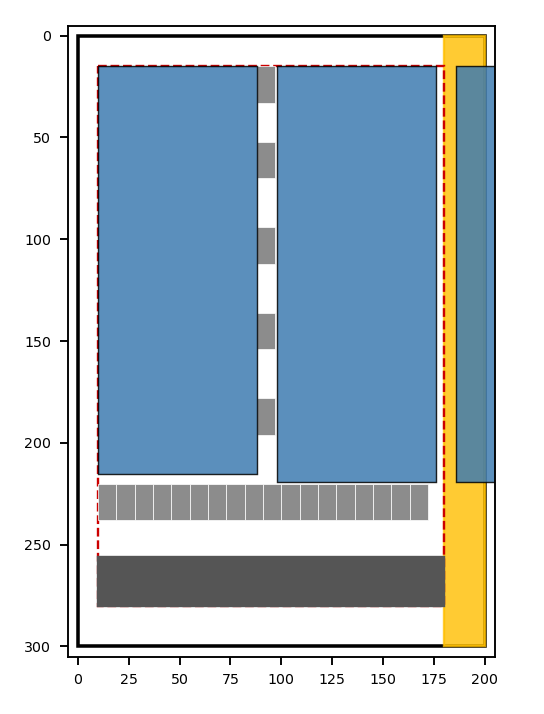
\includegraphics[width=\linewidth]{plan_0.png}\caption{\scriptsize Baseline: 4 floors, surface parking}\end{subfigure}
\begin{subfigure}{0.32\linewidth}\centering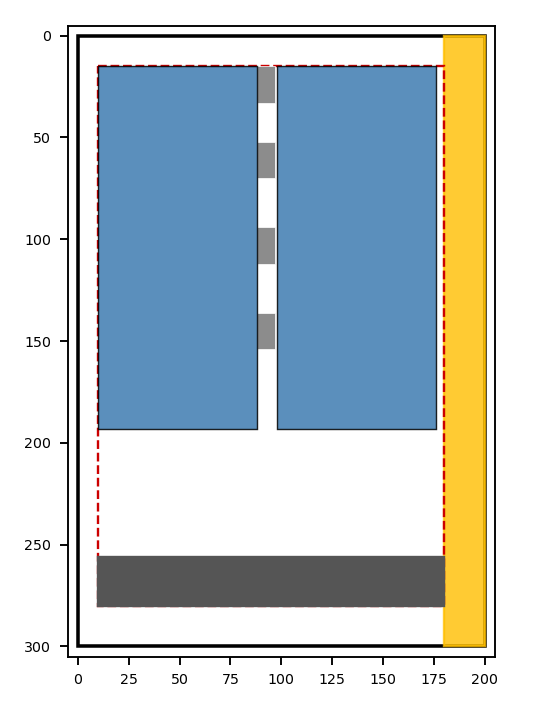
\includegraphics[width=\linewidth]{plan_1.png}\caption{\scriptsize Right-sized: 60 units, podium (compliant)}\end{subfigure}
\begin{subfigure}{0.32\linewidth}\centering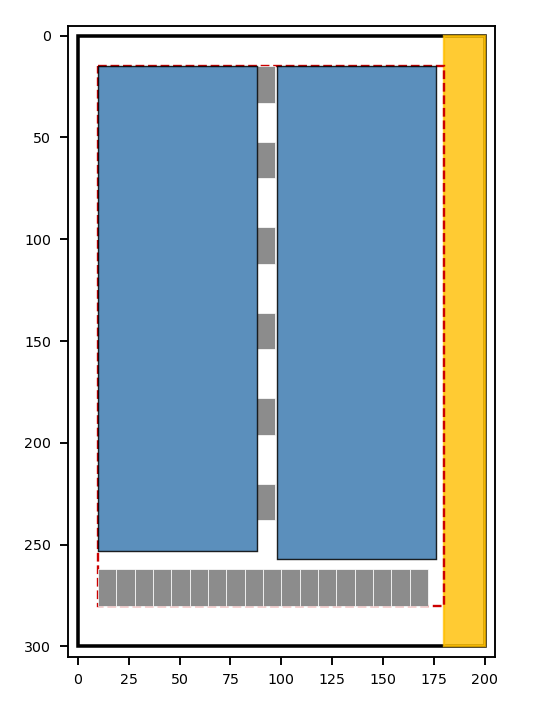
\includegraphics[width=\linewidth]{plan_2.png}\caption{\scriptsize Podium parking, 5 floors}\end{subfigure}
\caption{Top views (street at top; yellow = easement, dashed red = buildable envelope, grey = driveway and stalls, blue = building wings).}
\end{figure}
\begin{figure}[H]\centering
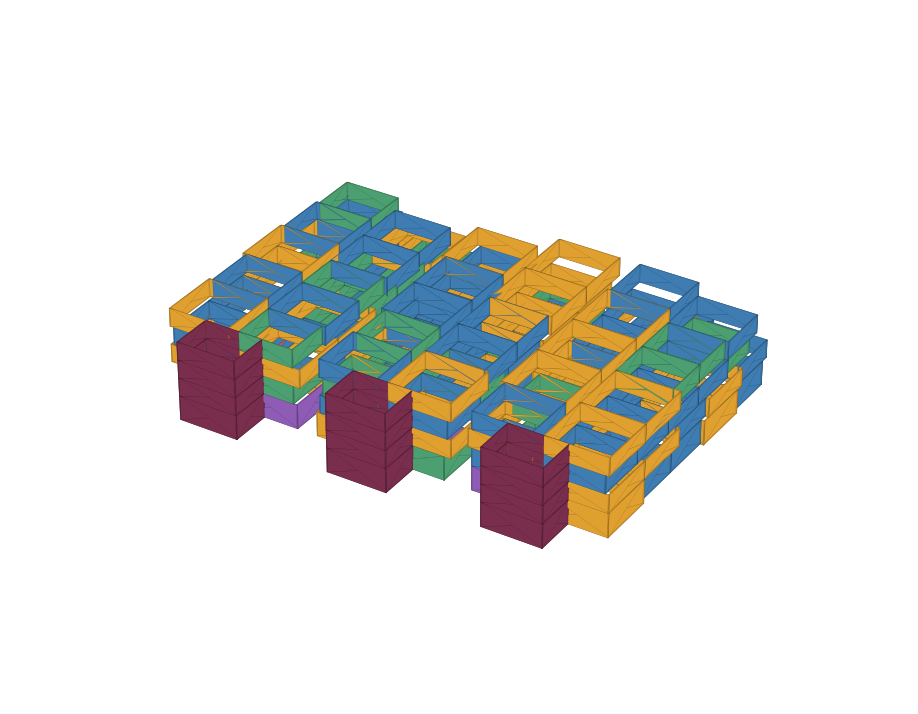
\includegraphics[width=0.48\linewidth]{view_0.png}\hfill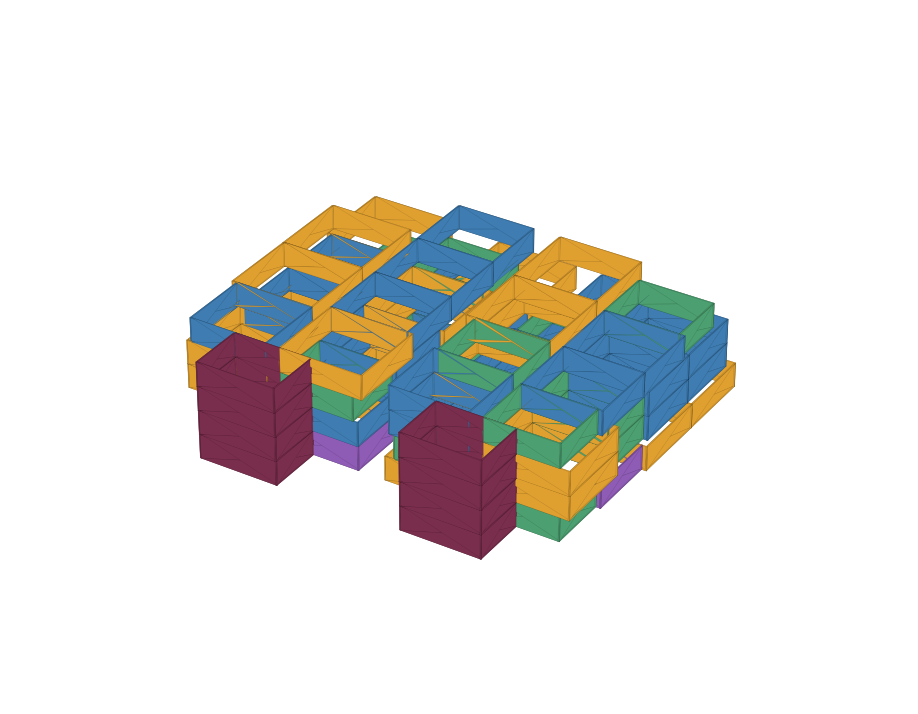
\includegraphics[width=0.48\linewidth]{view_1.png}
\caption{3D renders read back from the IFC files (walls colored by unit type): baseline 120 units (left) and the right-sized 60-unit podium design (right).}
\end{figure}

\subsection{Reading the scenarios}
\begin{itemize}
\item \textbf{Baseline (120 units, 4 floors, surface):} the units all fit, but three wings need more width than the envelope offers, coverage and FAR exceed the R-4 limits, and only a fraction of the 150 stalls fit. This is a program/site mismatch, not a layout bug.
\item \textbf{Right-sized (60 units, podium):} halving the program lets two wings fit inside the setbacks with a fire lane, and podium parking covers all 75 stalls. All ten checks pass.
\item \textbf{Podium, 5 floors (120 units):} more height cuts the footprint, but the podium level makes 6 stories and pushes height past the limit.
\item \textbf{Dense R-6:} looser coverage and parking rules help, but 7 floors plus a podium exceed the 7-story cap.
\item \textbf{Suburban R-2:} strict FAR (1.0) and coverage (40\,\%) fail even at 60 units, showing how the zoning preset alone can decide feasibility.
\end{itemize}

\begin{table}[H]\centering\footnotesize
\caption{Compliance checks, right-sized 60-unit podium design.}
\begin{tabular}{llll}\toprule Check & Required & Provided & Status \\ \midrule
Units placed & 60 & 60 & PASS \\
Stories & $\le$ 5 & 5 & PASS \\
Height (ft) & $\le$ 65 & 56.0 & PASS \\
FAR & $\le$ 2.5 & 2.31 & PASS \\
Lot coverage \% & $\le$ 60 & 46.3 & PASS \\
Parking stalls & 75 & 75 & PASS \\
Building inside setbacks/easement & yes & yes & PASS \\
Fire lane / driveway (24 ft) & yes & yes & PASS \\
Accessible units (2\%) & 2 & 2 & PASS \\
Exit travel to core (ft) & $\le$ 200 & 154 & PASS \\
\bottomrule\end{tabular}\end{table}
\begin{table}[H]\centering\footnotesize
\caption{Compliance checks, 120-unit baseline.}
\begin{tabular}{llll}\toprule Check & Required & Provided & Status \\ \midrule
Units placed & 120 & 120 & PASS \\
Stories & $\le$ 5 & 4 & PASS \\
Height (ft) & $\le$ 65 & 45.5 & PASS \\
FAR & $\le$ 2.5 & 3.16 & FAIL \\
Lot coverage \% & $\le$ 60 & 79.1 & FAIL \\
Parking stalls & 150 & 23 & FAIL \\
Building inside setbacks/easement & yes & no & FAIL \\
Fire lane / driveway (24 ft) & yes & yes & PASS \\
Accessible units (2\%) & 3 & 3 & PASS \\
Exit travel to core (ft) & $\le$ 200 & 180 & PASS \\
\bottomrule\end{tabular}\end{table}

\section{Testing}
\texttt{test\_design.py} contains 12 pytest tests, all passing:
\begin{itemize}[nosep]
\item module counts always sum to the requested units;
\item the right-sized scenario passes every check, and the baseline correctly fails parking;
\item more floors shrink the footprint; the Suburban preset reports FAR $\le 1.0$;
\item accessible units are created;
\item for every scenario: the IFC has the right number of storeys and at least four walls per unit, and triangulation succeeds (round-trip);
\item a headless Streamlit \texttt{AppTest} loads the app and clicks a scenario button.
\end{itemize}
One real bug was found in use: launching with \texttt{streamlit run app.py} from inside the folder crashed because \texttt{Path(\_\_file\_\_)} was a relative path. It was fixed by resolving the path, and the fix was checked by running the app with a relative path. Another problem found while writing this report was that early 3D renders showed only floors; walls-only rendering fixed it.

\section{Limitations and next steps}
\begin{itemize}
\item \textbf{Sample data.} Real jurisdiction rules and RNGD's real BaaP catalog must replace the synthetic ones (the code needs only new data files).
\item \textbf{Simple geometry.} Rectangular wings only; no L/U shapes, doors, windows, structure or MEP. Units are box walls.
\item \textbf{Approximate parking.} A free-space scan with no full aisle-geometry check, and a rule-of-thumb podium capacity.
\item \textbf{Proxy checks.} Fire lane, exit travel and accessibility are simplified stand-ins, not code determinations. A licensed professional must review any real design.
\item \textbf{Next steps.} Add L/U wings, doors and windows, structural grid alignment, IFC property sets (areas, unit IDs) for quantity take-off, and connect the real BaaP data.
\end{itemize}

\section{How to run}
\begin{verbatim}
cd Testt/ifc_design
pip install ifcopenshell plotly
streamlit run app.py            # browser app (Chrome)
python generate.py              # writes out/*.ifc and out/*.html
python -m pytest test_design.py # 12 tests
python build_report.py          # rebuilds this PDF
\end{verbatim}
Open any \texttt{out/*.html} by double-clicking; open any \texttt{out/*.ifc} in BIMvision, Blender-BIM, FreeCAD or the free Autodesk Viewer.
\end{document}
